\subsection{Victron system}\label{sec:Victron}
The Victron system is a commercial device that will be placed in the e-bike charging station. It consists of all the necessary power electronics, except for the physical chargers for the e-bikes. Hence the system contains the inverter for the solar panels (BlueSolar), batteries to store the energy and power electronics to control the distribution of power (MultiPlus). It is also possible to extract or deliver energy to the grid if needed. Inside the Victron there is a component called the Color Control GX \cite{GXPanel} or CCGX, which is used as a simple panel that displays data and settings. All components in the Victron system are connected to this Color Control. 

\begin{figure}[!ht]
  \centering
    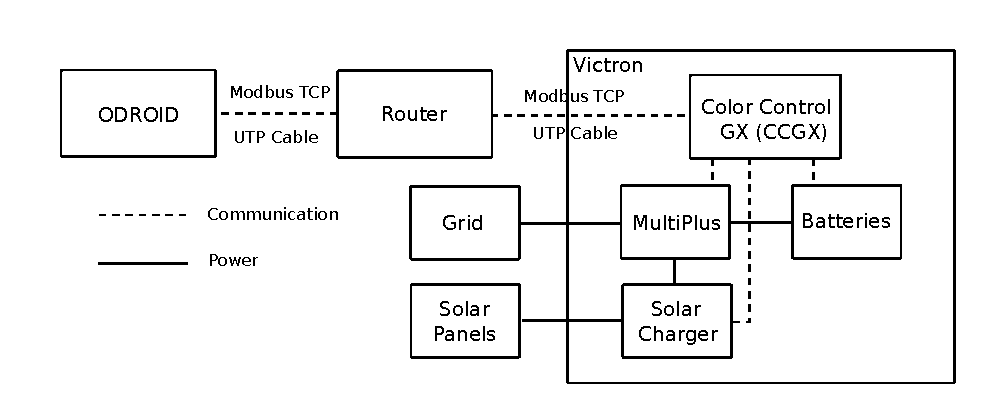
\includegraphics[width=1.0\textwidth]{images/victron.pdf}
      \caption{Overview of the Victron system}\label{fig:victron}
\end{figure}

\Cref{fig:victron} shows the configuration of the Victron system with the power connections, as well as connections for communication. In order to read data from the Victron system \ref{eis:1.2}, it must be connected to a network. This is done using a UTP cable which is connected to a router. The ODROID is connected to this router as well. Using Modbus TCP the ODROID can communicate with the Victron system and read it's registers.

\subsubsection{Reading the registers}
Reading registers is mainly based on the register list made by Victron Energy \cite{excel_registers}. Each entry in this list corresponds to a register that can be read.

\begin{table}
\centering
\caption{Part of register list of Victron Energy \cite{excel_registers}}
\begin{tabular}{|l|l|l|l|l|l|}
\hline
\textbf{dbus-service-name} & \textbf{Description}  & \textbf{Address} & \textbf{Type} & \textbf{Scalefactor} & \textbf{dbus-unit} \\ \hline
com.victronenergy.vebus    & Input voltage phase 1 & 3                & uint16        & 10                   & V AC               \\ \hline
com.victronenergy.battery  & Battery voltage       & 259              & uint16        & 100                  & V DC               \\ \hline
\end{tabular}
\label{reg_list}
\end{table}

Two entries from this list are shown in \Cref{reg_list}. The entire list contains 181 entries. Due to irrelevance some datafields of the two entries are omitted. It was decided that the registers 3-38 (MuliPlus), 259-303 (Battery) and 778-790 (Solar Charger) will be read. All other data will probably not be very relevant for this project. It is worth noting that the registers are not ordered from 0-180, but in blocks of register addresses. E.g. the first block has address 3 to 41, whereas the second block has address 259 to 304 (compensating for this offset is explained in more detail in \Cref{sec:offset}).\\

Using the Modbus libary for C, it is only possible to read registers between two register addresses, hence the data is read in four seperate function calls. Using the Modbus library functions these registers can be read by specifying a range of addresses and a slave ID. This slave ID is the ID of the seperate parts whithin the Victron system. On the CCGX monitor mounted on the Victron system a device instance number is shown for the connected devices. Using the second page of the register list \cite{excel_registers} this device instance number can be converted to a unit ID, which is equal to the slave ID needed for the Modbus function. For example, the device instance for the batteries is 256, which corresponds to unit ID 247.\\

Interstingly, the CCGX detects the MultiPlus as two seperate units. One MultiPlus unit on device instance 0 and one on device instance 257. The meaning of this is further explained in \Cref{sec:victron_results}.
%On device instance 0 the data regarding the external power sockets connected to the Victron system can be read. Currently, the ODROID, display and router are connected to these sockets. The same registers on device ID 257 contain the information about the internal power consumption of the Victron.\\
%Gedeelte over internal consumption evt. nog uitbreiden.

\subsubsection{Robustness}
In order to keep the code robust \ref{eis:2.3}, the code detects three different types of errors: an invalid register number is requested, the Modbus TCP connections failed or reading of a register failed (these are all similar to the checks explained in \Cref{sec:weather_robustness}). For robustness it is desired not to stop the program if a failure occurs, hence it is chosen to let the functions return a 0 if a failure occurs, after which a check is done on the validity of the fetch.\\

\scriptsize
	\lstinputlisting [language=C,caption=Code to detect if an error occured,label=script:victron] {code/victronread.c}
\normalsize

Script \ref{script:victron} shows that if an error occured, and a 0 is returned, no data will be sent to the server. In this way there are no errors caused in the code that sends the data to the server and the program can keep running.\\

\subsubsection{Flexibility and offset}\label{sec:offset}
In the future it could be desired to read other registers than the registers chosen for this design. To still be able to use the code, it was chosen to implement some flexibility. For example the file \verb|scaleTables.c| contains the scalefactor and datatype of all registers instead of only those read in the current program. However, since the registers are not addressed as 0 to 180, a conversion is needed from the register address to the index of the vector containing scalefactor and datatype. This is done using a variable called \verb|offset|.

\scriptsize
	\lstinputlisting [language=C,caption=Select offset from registeraddress,label=script:offset_select] {code/offset_select.c}
\normalsize

Script \ref{script:offset_select} shows how the offset is selected from the register address. All addresses are mapped onto the range ${0,1,...,180}$. Now this offset can be used for the scaling and casting purposes explained below. Also note that the last 4 lines return a 0 if the register address does not exist. Furthermore, it is desired to determine the slave ID based on the requested register address. However, there are two MultiPlus instances hence the same register addresses can be read at different slave IDs. Therefore, the slave ID cannot be uniquely determined based on the requested register address. As a consequence the slave ID must be provided as function argument together with the addresses to be read.\\

\subsubsection{Casting register values}\label{sec:casting}
All data received from the Victron system is represented as a \verb|uint16_t|. However, not all the data is actually readable as a \verb|uint16_t| (values that can be positive or negative). Based on the datasheet \cite{excel_registers}, data is cast from \verb|uint16_t| to \verb|int|. This can be done directly for data that is of the type \verb|uint16_t| (See \Cref{fig:uint16_t}).\\

\begin{figure}[!ht]
  \centering
    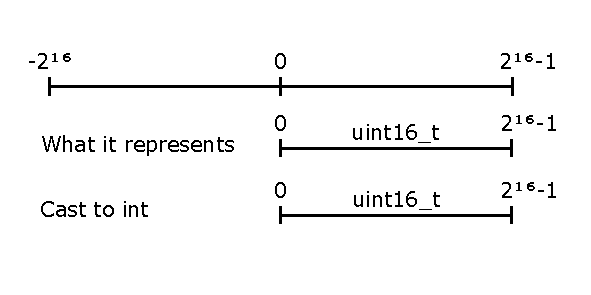
\includegraphics[width=0.5\textwidth]{images/Cast_voorbeeld_uint16_t.pdf}
      \caption{Casting a uint16\_t to int can be done without misinterpreting the information}\label{fig:uint16_t}
\end{figure}

Since the data of type \verb|int16_t| is also represented as a \verb|uint16_t| when received, casting will cause the MSB to be misinterpreted as part of the value instead of the sign (See \Cref{fig:int16_t}). To prevent this, the data has to be cast twice. First to \verb|int16_t|, and then to \verb|int|.\\

\begin{figure}[!ht]
  \centering
    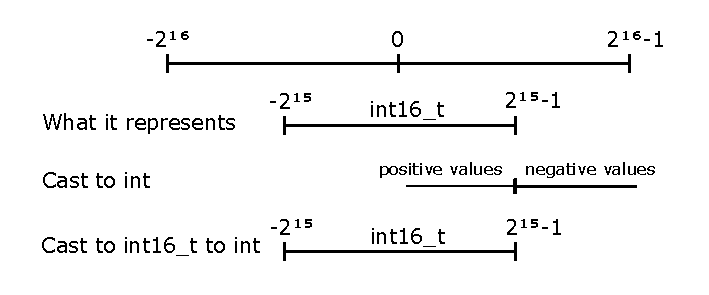
\includegraphics[width=0.6\textwidth]{images/Cast_voorbeeld_int16_t.pdf}
      \caption{Casting the uint16\_t to int causes a misintepretation of the sign bit. An extra cast to int16\_t is needed.}\label{fig:int16_t}
\end{figure}

The final casting diagram can be found in \Cref{fig:casting}. Any data that represents a string or \verb|int32| is not needed and therefore discarded.\\

\begin{figure}[!ht]
  \centering
    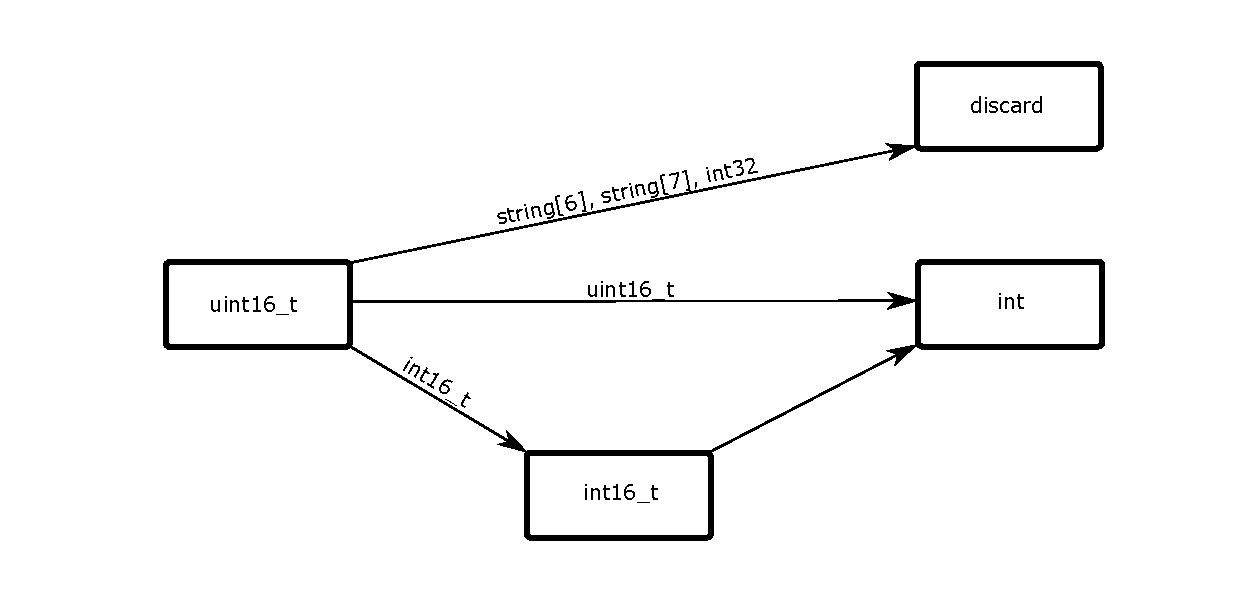
\includegraphics[width=\textwidth]{images/Cast_diagram.pdf}
      \caption{A diagram of how to cast certain data. The text close to the arrows describe how a certain register is logged in the Victron datasheet, the boxes show what type it is represented in. Note that 'discard' means that the value is not used in any further processing.}\label{fig:casting}
\end{figure}

The implementation of this casting sequence can be found in Script \ref{cast_code}. A seperate C-file (to keep things organized) holds the array which contains information about the type of data of a certain register. This array is made \verb|extern| so it can be called upon by functions outside of this file. The array elements correspond to the Victron registers in the same order as the datasheet by Victron Energy \cite{excel_registers}. The array is encoded, where '0' corresponds to a registers of type \verb|uint16_t| (line 9), '1' corresponds to a register of type \verb|int16_t| (line 13) and register values 2 to 4 correspond to values that are discarded (line 18). Discarded values are filled with zeroes so register values do not change of position in the array (line 22). The \verb|for|-loop will loop through all received data, followed by an \verb|if|-statement that checks how the register should be cast.

\scriptsize
	\lstinputlisting [language=C,caption=Cast function for Victron data,label=cast_code] {code/castVictronData.c}
\normalsize


%\scriptsize
%\begin{lstlisting}[language=C,caption={Cast function for Victron data},label={cast_code}]
%int* castVictronData(int start, int end, uint16_t *outputRegisters){
%
%	int regCount = end-start+1;
%	int *intOutputRegisters;
%
%	intOutputRegisters = (int *) malloc(regCount * sizeof(int));
%	memset(intOutputRegisters, 0, regCount * sizeof(int));
%
%	int i;
%	for (i = 0; i < regCount; i++){
%		// register is of type uint16_t
%		if (victronType[start+i] == 0){
%			intOutputRegisters[i] = (int) outputRegisters[i];
%		}
%		// register is of type int16_t
%		else if (victronType[start+i] == 1){
%			int16_t res = (int16_t) outputRegisters[i];
%			intOutputRegisters[i] = (int) res;
%		}
%		// ignore registers of type int 32, string[6], string[7]
%		else {//if (VictronType[start+i] == 2 || VictronType[start+i] == 3 || VictronType[start+i] == 4){
%			intOutputRegisters[i] = 0;
%		}
%	}
%	return intOutputRegisters;
%}
%\end{lstlisting}
%\normalsize

\subsubsection{Scaling register values}\label{sec:scaling}
Scaling is done in a similar way as casting of the values (see \Cref{sec:casting}). An array in a seperate C-file, called \verb|victronScale[]|, contains all the scale factors and is made of type \verb|extern double|. Register values are cast to \verb|double| and then divided by their corresponding scale factor (line 3 in Script \ref{scaling_code}). Note that values of \verb|victronScale| are called upon at an offset to ensure scaling by the correct value, this is explained in \Cref{sec:offset}.

\scriptsize
	\lstinputlisting [language=C,caption=Scaling function for Victron data,label=scaling_code] {code/scaleVictronData.c}
\normalsize

%\scriptsize
%\begin{lstlisting}[language=C,caption={Scaling function for Victron data},label={scaling_code}]
%for (i = 0; i < regCount; i++){
%		doubleOutputRegisters[i] = ((double)intOutputRegisters[i]) / victronScale[start-offset+i];
%}
%	\end{lstlisting}
%\normalsize